\documentclass[pmlr,twocolumn,10pt]{jmlr}

% Official ML4H 2026 Proceedings review configuration.
\mlhtrack{proceedings}
\newif\iffinal
\finalfalse

\iffinal
  \ifmlhneedspmlr
    \jmlrvolume{XXX}
    \jmlryear{2026}
  \fi
  \jmlrworkshop{Machine Learning for Health (ML4H) 2026}
\else
  \jmlrproceedings{}{Submitted to ML4H 2026: \mlhtrackname}
  \jmlrworkshop{Machine Learning for Health (ML4H) 2026}
\fi

% The class loads amsmath, amssymb, natbib, graphicx, url, and algorithm2e.
\urlstyle{same}
\usepackage{booktabs}
\usepackage{siunitx}
\usepackage[switch]{lineno}

\hypersetup{
  pdftitle={SLICES: A Benchmark and Evaluation Framework for Self-Supervised Learning on Sparse ICU Time Series},
  pdfauthor={},
  pdfsubject={ML4H 2026 Proceedings submission},
  pdfkeywords={self-supervised learning, intensive care, time series, benchmark}
}

\newcommand{\SLICES}{SLICES}
\newcommand{\MIMIC}{MIMIC-IV}
\newcommand{\EICU}{eICU-CRD}
\newcommand{\Combined}{Combined}
\newcommand{\MAE}{MAE}
\newcommand{\JEPA}{JEPA}
\newcommand{\Con}{Contrastive}
\newcommand{\FT}{Fine-tune}
\newcommand{\LP}{Probe}
\newcommand{\NA}{--}
\defcitealias{kdigo2012aki}{KDIGO AKI Work Group, 2012}

\title[SLICES: Benchmarking SSL on Sparse ICU Time Series]{SLICES: A Benchmark and Evaluation Framework for Self-Supervised Learning on Sparse ICU Time Series}
\author{Anonymous Author(s)}

\linenumbers

\begin{document}
\maketitle

\begin{abstract}
Self-supervised learning (SSL) results for intensive care unit (ICU) time series are hard to compare when data processing, encoders, and adaptation vary together. We present \SLICES{}, a benchmark and evaluation framework for comparing and extending SSL methods under a shared clinical setup. It fixes 24-hour value--observation-mask inputs, a Transformer encoder, patient-level splits, four endpoints, two adaptation protocols, and five matched seeds across \MIMIC{}, \EICU{}, and their pooled union. Masked autoencoding (\MAE{}), joint-embedding prediction (\JEPA{}), and contrastive learning provide reference implementations. \MAE{} leads mean AUPRC in all nine frozen classification comparisons and seven of nine fine-tuning comparisons among SSL methods. This advantage depends on the endpoint. Frozen \MAE{} has higher mean length-of-stay absolute error than a constant training-median predictor in all three regimes, and supervised or classical baselines lead selected endpoints. The code repository supports new objectives, shared downstream evaluation, and regeneration of the reference results. \SLICES{} thus provides both a reusable comparison framework and evidence that SSL choices depend on the task and adaptation protocol. Comparisons remain descriptive and implementation-specific, with equal data passes but unequal compute and tuning effort.
\end{abstract}

\begin{keywords}
self-supervised learning, clinical time series, intensive care, benchmark, missing data
\end{keywords}

\ifmlhneedsstatements
\paragraph*{Data and Code Availability}
We use deidentified \MIMIC{} v2.2 and \EICU{} v2.0 data from PhysioNet under credentialed access \citep{physionet2023mimiciv22,physionet2019eicu20}. The accompanying code repository contains run-level aggregate results and executable audits. It excludes patient records, split identities, credentials, and trained patient-data weights. Aggregate auditing needs no data access. Training reproduction requires independent credentialing, training, and a data-use agreement.
\fi

\section{Introduction}
\label{sec:introduction}

\begin{figure*}[!t]
\floatconts{fig:thesis-overview}
{\caption{Benchmark overview. Cohorts, hourly inputs, encoder architecture, patient splits, tasks, and evaluation protocols are fixed. SSL implementations vary in their masks and auxiliary modules. Equal epochs do not imply equal compute. Baselines provide context, and TS2Vec-style illustrates extension. LOS uses mean absolute error in days.}}
{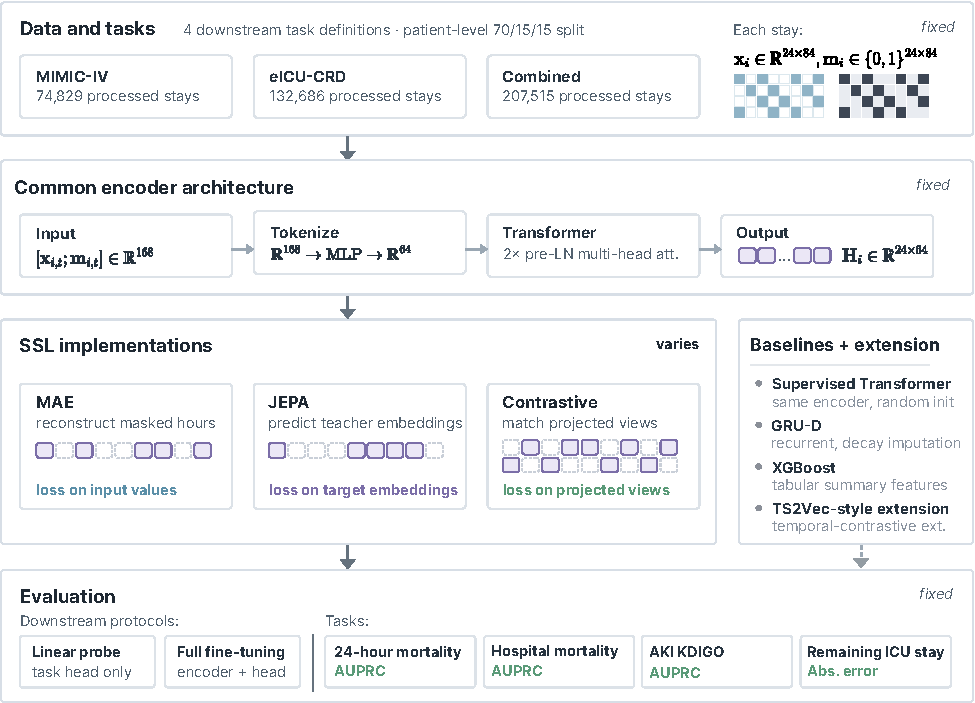
\includegraphics[width=.92\textwidth]{diagrams/fig01-benchmark-overview.pdf}}
\end{figure*}

ICU records are sparse because measurements are taken at different frequencies and often in response to a patient's evolving condition. The absence and timing of a measurement can therefore carry information about both physiology and care processes \citep{tan2023informativemissingness}. This makes ICU time series a relevant test bed for SSL: unlabeled measurements are abundant, yet the measurement process itself complicates the choice of learning signal.

Prior clinical SSL studies use reconstruction, forecasting, contrastive learning, or combined pretext tasks \citep{tipirneni2022strats,labach2023duett,yeche2021ncl,oufattole2024ebcl}. Their differences are hard to attribute when cohorts, representations, encoders, augmentations, and evaluation also vary. A systematic review of structured-EHR foundation models found similar heterogeneity in features, temporal representation, SSL objectives, and adaptation, with compute often underreported \citep{guo2026ehrfoundationreview}. Frozen probes test whether task information is linearly accessible. Fine-tuning tests whether a pretrained initialization remains useful after label-driven adaptation. Either alone can hide a protocol-dependent ranking.

\SLICES{} makes the evaluation contract reusable (Figure~\ref{fig:thesis-overview}). A new objective consumes the same value--mask tensors, returns a loss through a common interface, and exports the same encoder for downstream evaluation. A machine-readable specification and result validators make changes to the comparison explicit. The controlled unit is the complete implementation: masking geometry, auxiliary networks, encoder passes, and pretraining parameter counts remain objective specific.

Our contributions are:
\begin{enumerate}
  \item A fixed sparse-ICU benchmark specification and an objective/encoder-transfer interface, with MAE, JEPA, and contrastive reference implementations and a documented extension workflow.
  \item A code repository with the historical training implementation, framework code, checksummed aggregate results, and tools to regenerate results and check comparability without patient-data access.
  \item A reference evaluation built on a 2,455-run launch matrix across two databases and their union, using five matched seeds to examine objective choice, adaptation, label efficiency, transfer, capacity, and baseline performance.
\end{enumerate}

\section{Related Work}
\label{sec:related}

\paragraph{ICU benchmarks.}
The MIMIC-III benchmark formalized common ICU prediction tasks and evaluation procedures \citep{harutyunyan2019multitask}. YAIB provided a modular multi-center clinical framework over several ICU databases using harmonized preprocessing \citep{van_de_water2024yaib}. \SLICES{} builds on explicit cohorts, labels, and leakage controls with a setup designed for SSL comparisons. It holds the clinical inputs, encoder, and downstream evaluation fixed across objectives, reducing variation from these sources.

\paragraph{Clinical time-series SSL.}
STraTS represents sparse observations as time--variable--value triplets and uses forecasting-style pretraining \citep{tipirneni2022strats}. DuETT uses dual event-time attention and self-supervised prediction tasks \citep{labach2023duett}. Neighborhood and event-based contrastive methods use clinical structure to define positive pairs or anchors \citep{yeche2021ncl,oufattole2024ebcl}. Sequential multi-dimensional SSL evaluates contrastive and non-contrastive losses at multiple levels of clinical trajectories \citep{raghu2023smdssl}. SMART combines missing-aware temporal and variable attention with latent reconstruction \citep{yu2024smart}. AID-MAE is a recent masked-modeling approach for incomplete EHR time series \citep{xiang2026aidmae}. These systems motivate the objectives studied here but change either the representation, architecture, positive-pair rule, or task contract.

\paragraph{Closest comparative work.}
TS-JEPA compares JEPA, masked autoencoding, autoregression, and TS2Vec-style contrastive pretraining with a common Transformer, on sensor and forecasting datasets, with frozen-head evaluation and a low-label study \citep{ennadir2024tsjepa}. It is the closest objective-level predecessor. \SLICES{} differs in its missingness-preserving ICU interface, patient-level clinical splits, paired probe and fine-tuning evaluation, and matched \MIMIC{}--\EICU{} regimes. Clin-JEPA uses text-serialized hourly states and an LLM-based encoder, so it changes the model and input contract rather than testing a shared small-encoder interface \citep{yang2026clinjepa}. General MAE, I-JEPA, SimCLR, and TS2Vec formulations provide the objective context \citep{he2022mae,assran2023ijepa,chen2020simclr,yue2022ts2vec}.

SLICES combines modular clinical evaluation with a shared-encoder SSL comparison. Its specific contribution is the reusable sparse-ICU evaluation contract, paired frozen and fully adapted evaluations, and traceable result package. Scores remain study-specific because cohorts, representations, and tasks differ.


\section{Benchmark Design}
\label{sec:design}

\subsection{Cohorts and Hourly Representation}

We use \MIMIC{} v2.2 and \EICU{} v2.0 \citep{johnson2023mimiciv,pollard2018eicu}. Common extraction and unit harmonization are based on RICU \citep{bennett2023ricu}. Each sample is one ICU stay with valid patient and stay metadata, ICU duration of at least 24 hours, and at least one observed time-series value in the first 24 hours. The processed cohorts contain 74,829 \MIMIC{} stays and 132,686 \EICU{} stays. We form their 207,515-stay union, \emph{Combined}, after schema compatibility checks and source-specific identifier namespacing. It is a pooled training regime, not an independent cohort.

Each stay is represented as normalized values $x\in\mathbb{R}^{24\times84}$ and an observation mask $m\in\{0,1\}^{24\times84}$. Feature means and standard deviations are fitted on the training partition only. Missing cells are zero filled after normalization while $m$ preserves whether a value was observed. The 84 retained variables are shared across data regimes. Only 10.7\% to 15.3\% of tensor cells are observed, although most stays have at least one measurement in nearly every hour. This distinction matters: temporal coverage is high, but within-hour feature coverage remains sparse.

Patients are assigned to 70/15/15 train, validation, and test partitions for each seed. All stays for one patient remain in one partition. Task-specific missing labels are removed only after this assignment, and the same split is used for pretraining and downstream evaluation. Input normalization uses training data only. Direct length-of-stay variables, future-duration helpers, and derived features that expose downstream outcomes are excluded from the input.

\subsection{Endpoints and Horizons}

All tasks use the first 24 ICU hours as input. Classification uses area under the precision--recall curve (AUPRC), computed as average precision, because prevalence is low and endpoint dependent \citep{saito2015precisionrecall}. Mean test prevalence spans 1.6\%--20.3\% (\tableref{tab:test-support}). Twenty-four-hour mortality predicts death in hours 24--48. Hospital mortality predicts in-hospital death after hour 24. Deaths within the input window receive null labels. Creatinine-defined AKI uses the minimum in hours 0--24 as baseline and seeks KDIGO stage~$\geq1$ evidence in hours 24--48: a later value at least 1.5 times baseline or at least 0.3 mg/dL above an earlier value within 48 hours \citepalias{kdigo2012aki}. Urine output is excluded. A missing baseline or forward measurement yields a null label. Remaining ICU length of stay (LOS) is ICU duration minus one day, clipped at zero. We retain this continuous target rather than impose a binary threshold. Absolute error keeps prediction misses interpretable in days.


\begin{figure*}[t]
\floatconts{fig:ssl-objectives}
{\caption{Core objective geometries. MAE reconstructs observed values at masked hours. JEPA's online encoder receives visible valid hours. Its EMA target encoder receives the full unmasked valid sequence. JEPA predicts layer-normalized, stop-gradient targets, with loss only on masked valid hours. Contrastive learning aligns projected pooled views. Auxiliary modules are discarded before downstream transfer.}}
{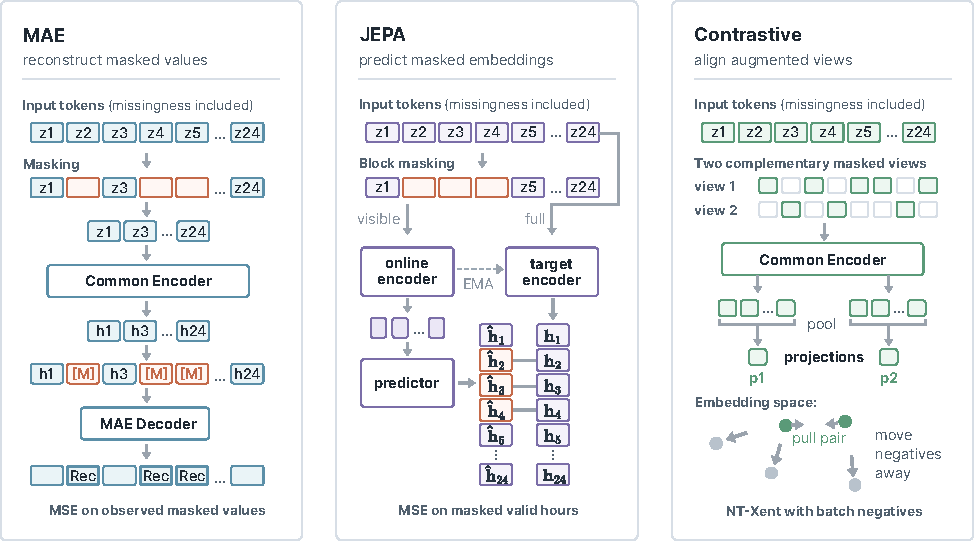
\includegraphics[width=\textwidth]{diagrams/fig04-ssl-objectives.pdf}}
\end{figure*}

\subsection{Shared Encoder and Objective-Specific Components}

Appendix Figure~\ref{fig:encoder-tokenization} shows the shared interface. Each hour is one continuous attention token: 84 normalized values and 84 observation indicators are concatenated and projected from $\mathbb{R}^{168}$ to $\mathbb{R}^{64}$, without value quantization or vocabulary lookup. The shared small Transformer has sinusoidal time encoding, two pre-layer-normalized layers, four heads, feed-forward width 256, and dropout 0.1. Empty hours are excluded from attention and SSL losses. Downstream heads mean-pool valid outputs. The same 159,808-parameter encoder transfers for every SSL method.

Figure~\ref{fig:ssl-objectives} contrasts the learning signals. \MAE{} masks random non-empty hours, encodes visible tokens, and uses a lightweight decoder to reconstruct observed normalized values at masked hours. Missing cells do not enter the loss. \JEPA{} masks up to three contiguous blocks. An online encoder and predictor estimate layer-normalized embeddings from a stop-gradient exponential-moving-average target encoder. Contrastive learning makes two complementary masked views, encodes each separately, mean-pools visible hours, and applies an MLP projection with an NT-Xent instance loss at temperature 0.07. Only the common encoder transfers downstream.

The implementations preserve reconstruction, latent prediction, and view agreement as distinct learning signals while sharing inputs, transferred encoder, and evaluation. Objective-specific masks and auxiliary modules retain each method's learning structure. MAE has 269,460 trainable pretraining parameters, JEPA has 189,440 plus a non-trainable 159,808-parameter target copy, and contrastive learning has 193,408 with two encoder passes. These are comparisons of complete implementations, not causal loss-function effects.

\begin{table}[!htbp]
\floatconts
  {tab:pretraining}
  {\caption{Core pretraining contract. Ratio is the configured timestep-mask ratio. All rows use AdamW, batch size 256, 100 epochs, and the same transferred encoder.}}
  {\scriptsize
  \begin{tabular}{llll}
  \toprule
  Objective & Masking & Target & Ratio \\
  \midrule
  \MAE{} & random hours & observed values & .5 \\
  \JEPA{} & $\leq3$ blocks & target embeddings & .5 \\
  Contrastive & two views & view agreement & .5 \\
  \bottomrule
  \end{tabular}}
\end{table}

\section{Experimental Setup}
\label{sec:setup}

\subsection{Using and Extending the Benchmark}
\label{sec:resource}

The code repository supports auditing reference results, reproducing the comparison with credentialed data access, and evaluating additional SSL objectives (Appendix Figure~\ref{fig:benchmark}). A machine-readable specification records clinical inputs, splits, tasks, encoder, training and checkpoint policies, and metrics. Comparability checks flag changed settings.

New objectives use the shared value--mask input and export an encoder for both frozen probing and fine-tuning. Pretraining retains hourly representations. Downstream evaluation averages valid hours into one stay-level vector because each endpoint assigns one target to a stay. Auxiliary pretraining networks are discarded. The TS2Vec-style extension demonstrates this path. A short run on artificial data checks the workflow without patient-data access. Its scores are not clinical evidence. Appendix~\ref{app:extension-workflow} gives implementation and validation details.

Researchers can verify frozen run aggregates and regenerate tables and figures without retraining. Historical source, current framework, reference results, and later diagnostics remain separately traceable.

\subsection{Reference Evaluation}

The reference program comprises a 2,455-run launch matrix: 145 pretraining runs and 2,310 exported downstream or baseline evaluations. It tests objective and protocol choice, reduced-label performance, cross-database adaptation, hyperparameter and encoder-capacity sensitivity, classical baselines, and the TS2Vec-style extension. The core comparison accounts for 45 pretraining runs and 420 evaluations. Subgroup metrics are additional evaluation outputs. Secondary analyses broaden the questions without changing the core ranking.

\paragraph{Pretraining.}
All methods use 100 epochs, batch size 256, AdamW learning rate $10^{-3}$, weight decay .01, gradient clipping at 1.0, ten warmup epochs, and cosine decay to $10^{-6}$. There is no pretraining early stopping. Batches contain only training-partition stays. Validation loss is monitored, and the test partition is not used. Equal epochs give an equal data-pass schedule within each regime, not equal FLOPs, wall time, or objective-specific module cost. Configurations were fixed before the final rerun and reused across datasets, but were informed by prior implementation development. The benchmark is neither preregistered nor matched for tuning effort.

\paragraph{Adaptation.}
Frozen probing trains a linear head for at most 50 epochs with learning rate $10^{-4}$ while keeping the encoder fixed. Full fine-tuning trains the encoder and a width-64 ReLU head for at most 100 epochs with learning rate $3\times10^{-4}$. Both use batch size 64, weight decay .05, cosine scheduling, gradient clipping at 1.0, and validation patience 10. Neural classification uses square-root-balanced class weights and label smoothing of $0.1$. LOS trains with mean squared error but uses mean absolute error in days for evaluation and checkpoint selection. Classification checkpoint selection maximizes validation AUPRC. The two protocols differ in trainable scope, head capacity, learning rate, and epoch cap. Their scores are reported as distinct evaluations, not a freeze-only ablation.

\paragraph{Baselines.}
The supervised Transformer uses the same encoder family and full-fine-tuning trainer from random initialization. GRU-D provides a recurrent, missingness-aware comparator \citep{che2018grud}. XGBoost uses per-variable summary features, including extrema, first and last values, counts, and observation fractions \citep{chen2016xgboost}. TS2Vec is a temporal-contrastive extension, not a fourth core objective.

\paragraph{Seeds, metrics, and checkpoints.}
All reported core cells contain five runs with matched seeds. A seed jointly determines the patient split and stochastic training. We report mean and sample standard deviation across runs. These reruns describe split and training variation, not patient- or population-level uncertainty. All comparisons are descriptive, without confirmatory significance claims.

Every downstream SSL run starts from the encoder saved after the final pretraining epoch. It does not select a pretrained encoder using objective-specific validation loss. This gives all objectives the same 100-epoch data-pass rule but may disadvantage an objective whose useful representations peak earlier. Downstream and baseline test metrics use validation-selected downstream checkpoints. A separate two-task \MIMIC{} probe check found small mean differences between final and best-SSL-validation encoders for MAE and contrastive learning, while that selection worsened JEPA (Appendix~\ref{app:diagnostics}).

\section{Results}
\label{sec:results}

\subsection{Core Classification Results}

\tableref{tab:classification} reports all full-label classification cells. Under linear probing, \MAE{} has the highest mean AUPRC in all nine cells. This ordering holds in all 90 matched-seed comparisons against JEPA and contrastive learning. Mean paired advantages over the stronger SSL alternative range from .026 to .084 AUPRC. Appendix Figure~\ref{fig:seed-differences} shows the observed paired ranges. Fine-tuning differences often cross zero. Under fine-tuning, the SSL ranking is less uniform: \MAE{} leads seven cells, \JEPA{} leads \Combined{} AKI by .000054 AUPRC, and contrastive learning leads \MIMIC{} 24-hour mortality. Including the supervised Transformer changes the AKI result: supervised training has the highest mean in all three AKI cells.

\begin{table*}[t]
\floatconts
  {tab:classification}
  {\caption{Core classification AUPRC, mean (sample SD) over five matched seeds. Bold marks the highest unrounded mean in each row. The supervised Transformer is defined only for full fine-tuning.}}
  {\scriptsize
  \begin{tabular}{lllrrrr}
\toprule
Data & Protocol & Endpoint & MAE & JEPA & Contrastive & Supervised \\
\midrule
Combined & Fine-tune & 24h mortality & \textbf{0.409 (0.024)} & 0.391 (0.031) & 0.399 (0.029) & 0.389 (0.021) \\
Combined & Fine-tune & Hospital mortality & \textbf{0.531 (0.010)} & 0.521 (0.009) & 0.514 (0.016) & 0.518 (0.008) \\
Combined & Fine-tune & AKI & 0.626 (0.004) & 0.626 (0.005) & 0.614 (0.004) & \textbf{0.652 (0.003)} \\
Combined & Probe & 24h mortality & \textbf{0.284 (0.031)} & 0.188 (0.018) & 0.205 (0.016) & -- \\
Combined & Probe & Hospital mortality & \textbf{0.470 (0.013)} & 0.357 (0.006) & 0.392 (0.010) & -- \\
Combined & Probe & AKI & \textbf{0.447 (0.006)} & 0.327 (0.005) & 0.396 (0.005) & -- \\
eICU-CRD & Fine-tune & 24h mortality & \textbf{0.377 (0.013)} & 0.363 (0.008) & 0.360 (0.016) & 0.351 (0.022) \\
eICU-CRD & Fine-tune & Hospital mortality & \textbf{0.495 (0.005)} & 0.471 (0.007) & 0.471 (0.003) & 0.474 (0.004) \\
eICU-CRD & Fine-tune & AKI & 0.519 (0.017) & 0.515 (0.018) & 0.494 (0.012) & \textbf{0.554 (0.014)} \\
eICU-CRD & Probe & 24h mortality & \textbf{0.276 (0.015)} & 0.199 (0.017) & 0.195 (0.009) & -- \\
eICU-CRD & Probe & Hospital mortality & \textbf{0.439 (0.006)} & 0.355 (0.004) & 0.350 (0.010) & -- \\
eICU-CRD & Probe & AKI & \textbf{0.361 (0.009)} & 0.268 (0.008) & 0.286 (0.004) & -- \\
MIMIC-IV & Fine-tune & 24h mortality & 0.451 (0.045) & 0.451 (0.050) & \textbf{0.456 (0.042)} & 0.449 (0.032) \\
MIMIC-IV & Fine-tune & Hospital mortality & \textbf{0.579 (0.011)} & 0.564 (0.009) & 0.568 (0.011) & 0.565 (0.008) \\
MIMIC-IV & Fine-tune & AKI & 0.667 (0.009) & 0.642 (0.009) & 0.645 (0.009) & \textbf{0.693 (0.013)} \\
MIMIC-IV & Probe & 24h mortality & \textbf{0.312 (0.042)} & 0.236 (0.028) & 0.254 (0.035) & -- \\
MIMIC-IV & Probe & Hospital mortality & \textbf{0.510 (0.014)} & 0.415 (0.020) & 0.458 (0.023) & -- \\
MIMIC-IV & Probe & AKI & \textbf{0.504 (0.009)} & 0.410 (0.017) & 0.478 (0.009) & -- \\
\bottomrule
\end{tabular}
}
\end{table*}


\subsection{Length of Stay and Protocol Dependence}

The LOS ranking reverses part of the classification pattern. Contrastive learning has the lowest probe absolute error in all three regimes: 2.309, 2.139, and 2.592 days for \Combined{}, \EICU{}, and \MIMIC{}. The exported training-median constant has errors of 2.403, 2.176, and 2.733 days. Frozen \MAE{} is worse than this constant in all three mean comparisons, by .022, .015, and .022 days, respectively (\tableref{tab:los}). This is a mean ordering, not an all-seed claim. Fine-tuned \MAE{} leads \Combined{} and \EICU{}. Contrastive learning leads \MIMIC{}. The contrastive probes nevertheless have negative mean $R^2$ on \EICU{} and \Combined{}. Their advantage is specific to absolute error. Squared-error training and absolute-error evaluation target different conditional summaries.

\begin{table*}[t]
\floatconts
  {tab:los}
  {\caption{Remaining-LOS absolute error in days, mean (sample SD), $n=5$. Lower is better. The constant predicts each seed's training-label median. Duplicate logs are collapsed by dataset and seed. Bold selects the lowest model mean within a protocol, not a significance claim.}}
  {\scriptsize
  \begin{tabular}{llrrrrr}
\toprule
Data & Protocol & MAE & JEPA & Contrastive & Supervised & Constant median \\
\midrule
Combined & Fine-tune & \textbf{2.118 (0.029)} & 2.135 (0.013) & 2.152 (0.024) & 2.190 (0.031) & 2.403 (0.025) \\
Combined & Probe & 2.425 (0.027) & 2.475 (0.023) & \textbf{2.309 (0.029)} & -- & 2.403 (0.025) \\
eICU-CRD & Fine-tune & \textbf{1.964 (0.017)} & 1.977 (0.034) & 2.008 (0.031) & 1.997 (0.030) & 2.176 (0.006) \\
eICU-CRD & Probe & 2.191 (0.011) & 2.249 (0.022) & \textbf{2.139 (0.011)} & -- & 2.176 (0.006) \\
MIMIC-IV & Fine-tune & 2.368 (0.051) & 2.371 (0.069) & \textbf{2.359 (0.069)} & 2.397 (0.066) & 2.733 (0.074) \\
MIMIC-IV & Probe & 2.755 (0.058) & 2.679 (0.070) & \textbf{2.592 (0.076)} & -- & 2.733 (0.074) \\
\bottomrule
\end{tabular}
}
\end{table*}

\subsection{Baseline Exceptions}

\tableref{tab:baseline-full} places the best full-fine-tuned SSL mean beside supervised Transformer, GRU-D, and XGBoost. GRU-D has the highest mean AUPRC for 24-hour mortality on all three data regimes. XGBoost leads AKI on all three. MAE has the highest hospital-mortality mean on all three regimes, including \EICU{} (.495 versus .484 for GRU-D). The best SSL LOS mean is lowest on \Combined{}, \EICU{}, and \MIMIC{}, although the eICU margin over supervised is .032 days and the \MIMIC{} margin over GRU-D is .035 days. These comparisons use aligned cohorts, splits, tasks, and metrics, but the models have different input summaries and inductive biases.


\subsection{Secondary Diagnostics}

Excluding full-label references leaves 33 reduced-label dataset--task--fraction cells per protocol. Among the three SSL implementations, \MAE{} leads 30/33 fine-tuning and 28/33 probe means. Including supervised training changes the fine-tuning count to 28/33. At 1\% labels for \Combined{} hospital mortality, \MAE{} exceeds supervised AUPRC by .033, with paired-difference SD .012. At 5\% labels for 24-hour mortality, the difference is .010 with SD .027. These overlapping cells are descriptive, not independent tests. Appendix Figure~\ref{fig:label-efficiency} shows hospital mortality. Appendix~\ref{app:secondary} gives all lowest-fraction MAE--supervised comparisons.

The TS2Vec-style extension has the better fine-tuning mean than core contrastive in 8/12 cells, while core contrastive leads all 12 probe cells. It is an adapted implementation, not original TS2Vec. A targeted MIMIC-IV 24-hour-mortality fine-tuning slice spans about .018 AUPRC across tested hyperparameters. Appendix~\ref{app:diagnostics} also reports JEPA representation diagnostics.

After source pretraining and target-label fine-tuning, MAE leads all four \MIMIC{}-to-\EICU{} tasks and three reverse-direction tasks by mean primary metric. On \MIMIC{} 24-hour mortality, medium and large MAE encoders exceed matched supervised mean fine-tuning AUPRC at all three tested label fractions. Subgroup audits show gaps with incomplete attribute coverage (Appendix~\ref{app:secondary}).

A separate five-seed MIMIC-IV cached-probe diagnostic compares final and best-SSL-validation encoders. MAE retains the hospital-mortality lead and contrastive the LOS lead under both policies in every seed. Best-validation JEPA worsens by .0406 AUPRC and .2638 LOS days on average, moving its LOS mean rank from second to third. This is checkpoint sensitivity within two tasks and frozen probing. The CPU reruns are distinct from historical scores (Appendix~\ref{app:diagnostics}).

A separate post-hoc random-encoder check is worse than SSL probes in 118/120 seed-level comparisons across \MIMIC{} and \EICU{}. A new CPU control on \MIMIC{} hospital mortality obtains .301 (.025) AUPRC from masks alone and .404 (.013) from flattened values plus masks. Both use five patient splits and validation-selected linear logistic models. Their short SGD schedule differs from the SSL probe trainer. These controls show accessible input signal but do not isolate representation quality or provide optimized linear baselines. They are stored separately from frozen results (Appendix~\ref{app:raw}).

\section{Discussion}
\label{sec:discussion}

\paragraph{What can be reused.}
Researchers can audit run aggregates or add an objective while retaining clinical inputs, encoder transfer, and evaluation. The results show why both uses matter: MAE leads frozen classification, yet its frozen LOS mean is worse than a constant. Different masking, augmentation, and encoder designs may change these rankings.

\paragraph{Why reconstruction may fit the interface.}
The tensor exposes a value and observation mask at each hour. MAE reconstructs observed cells, JEPA predicts an evolving target embedding, and core contrastive learning compares pooled stay vectors. An interface preference for reconstruction is one hypothesis for the classification ordering. The controls do not identify the learned information or establish that continuous values are better than quantization.

\paragraph{Health relevance.}
ICU measurement patterns are informative but ambiguous: an unmeasured laboratory value may reflect clinical judgment, workflow, availability, or data loss. Preserving the observation mask lets the encoder use this pattern without treating missing cells as observed zeros. It does not make missingness causal or transportable. A model can learn site-specific measurement policy as readily as physiology. Reporting separate database and pooled regimes is therefore more informative than relying on pooled data alone.

\paragraph{Evaluation practice.}
For comparable hourly value--mask inputs, MAE is a strong reference SSL baseline for classification, including reduced-label evaluation. Both probes and fine-tuning remain necessary because they test different representation properties. Supervised, recurrent, and tabular baselines establish whether the SSL ordering also matters for task performance. Pretraining checkpoint and cost policies must be explicit. Equal epochs do not imply equal compute, and checkpoint selection affected JEPA in the two-task diagnostic.

\section{Limitations}
\label{sec:limitations}

The benchmark holds clinical inputs and downstream evaluation fixed while retaining the components needed by each objective. Objective-specific heads, target networks, encoder passes, and trainable parameter counts therefore differ. This supports comparison of complete implementations but cannot isolate the causal effect of loss functions. Configurations reflect unequal development histories and a small targeted sensitivity analysis, not matched compute or tuning budgets or objective-specific optima.

Fixing one continuous-valued hourly interface makes the objective comparison tractable, but rankings may change with quantized-value, event-token, or patch-based representations. Waveforms, notes, images, and full medication histories are out of scope. Selected medication rates and indicators remain hourly features. Shared masked views may underrepresent contrastive methods that rely on clinically defined positive pairs. \Combined{} is the union of \MIMIC{} and \EICU{}, not an external cohort. Cross-database analyses fine-tune on target labels rather than test zero-shot transfer. Both databases are retrospective and deidentified. Database shift, label construction, missingness, and care practice limit transportability.

Five matched seeds are few and reuse overlapping source populations. They describe split and optimization variation but do not establish population uncertainty, statistical equivalence, calibration quality, subgroup fairness, clinical utility, or deployment readiness. No confirmatory significance claim is made. The forward AKI label uses creatinine only and is not a full clinical KDIGO assessment. Final-epoch pretraining checkpoints may miss better earlier states, especially for a moving \JEPA{} target. The random-encoder check and short raw/mask control are post hoc. The latter covers one endpoint and database, uses a different optimizer, and does not establish a tuned linear baseline.

These choices provide a reproducible starting point for new objectives. Broader claims require matched tuning and compute, alternative representations, and external validation.

\section{Ethics, Access, and Reproducibility}
\label{sec:ethics}

The study analyzes retrospective, deidentified ICU records under the credentialing and data-use terms of PhysioNet. It involves no prospective intervention, patient contact, or automated clinical decision. Researchers seeking to reproduce the study must obtain their own \MIMIC{} and \EICU{} access and may not receive patient-level records from the authors.

The main reference results derive from the unchanged frozen export. Random-encoder, JEPA/checkpoint, and raw/mask diagnostics are distinct sources. The code repository records source digests and retained result columns, supports aggregate auditing, and provides an extension example that runs without patient data. Full credentialed preprocessing and historical training have not been rerun for this submission, so numerical retraining equivalence remains unverified.


\section{Conclusion}
\label{sec:conclusion}

\SLICES{} provides a fixed sparse-ICU benchmark specification, interchangeable SSL objectives, shared downstream evaluation, and auditable reference results. Its code repository supports result regeneration and objective extension without patient-data access. The reference evaluation supports MAE as a strong classification baseline under this hourly interface, including when labels are scarce. LOS, adaptation, and strong non-SSL baselines limit broader claims. Paired frozen and fine-tuned evaluation makes these differences visible. The framework supports testing new objectives, representations, and compute-matched training as separately traceable comparisons.

\typeout{ML4H-MAIN-END-PAGE:\thepage}
\clearpage

\bibliography{references}

\appendix
\section{Additional Benchmark Details}
\label{app:benchmark}


\subsection{Benchmark and Data Flow}

Figure~\ref{fig:data-pipeline} details the preprocessing path introduced in Figure~\ref{fig:thesis-overview}. Combined pools the two source databases. It is not an external cohort. The varying unit includes objective-specific masks, auxiliary modules, and compute.

\begin{figure*}[p]
\floatconts{fig:data-pipeline}
{\caption{Data pipeline. RICU supplies concept-specific harmonization and hourly aggregation. SLICES applies cohort and feature filters and forms values, masks, and labels. Patient assignment precedes task-specific null-label filtering. Normalization uses observed training cells, followed by zero filling with the observation mask retained. Event rows are illustrative.}}
{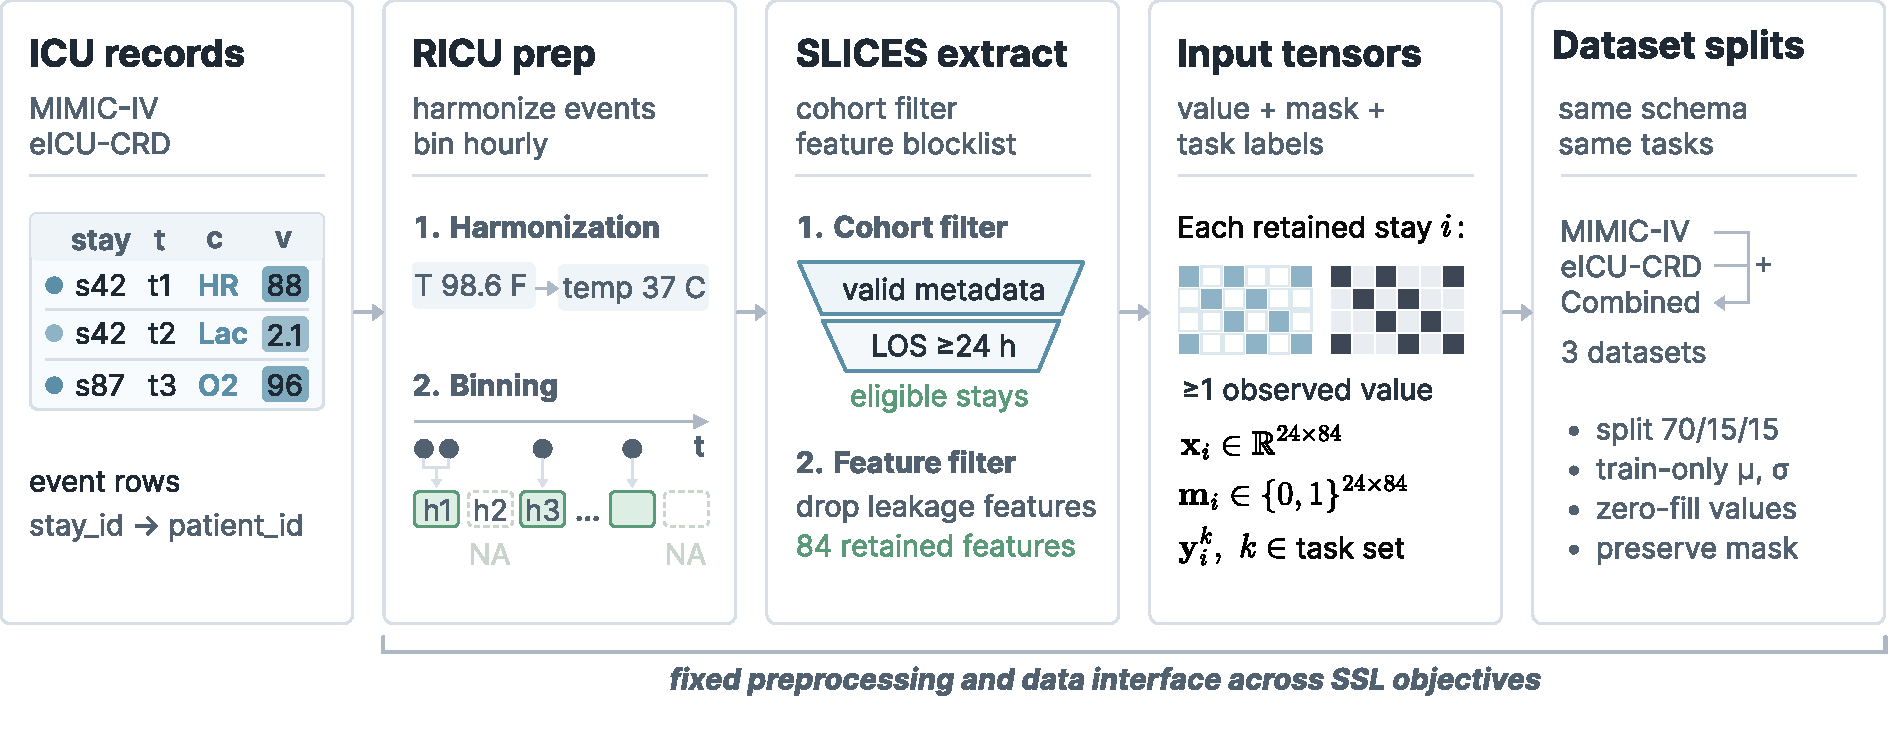
\includegraphics[width=\textwidth]{diagrams/fig02-data-pipeline.pdf}}
\end{figure*}

\begin{figure*}[p]
\floatconts{fig:encoder-tokenization}
{\caption{Shared hourly tokenization and encoder. Values and masks form 168 inputs per hour, projected to 64 dimensions. Empty hours are excluded from attention and losses. SSL uses timestep outputs, with objective-specific pooling for contrastive learning. Downstream heads mean-pool valid hours.}}
{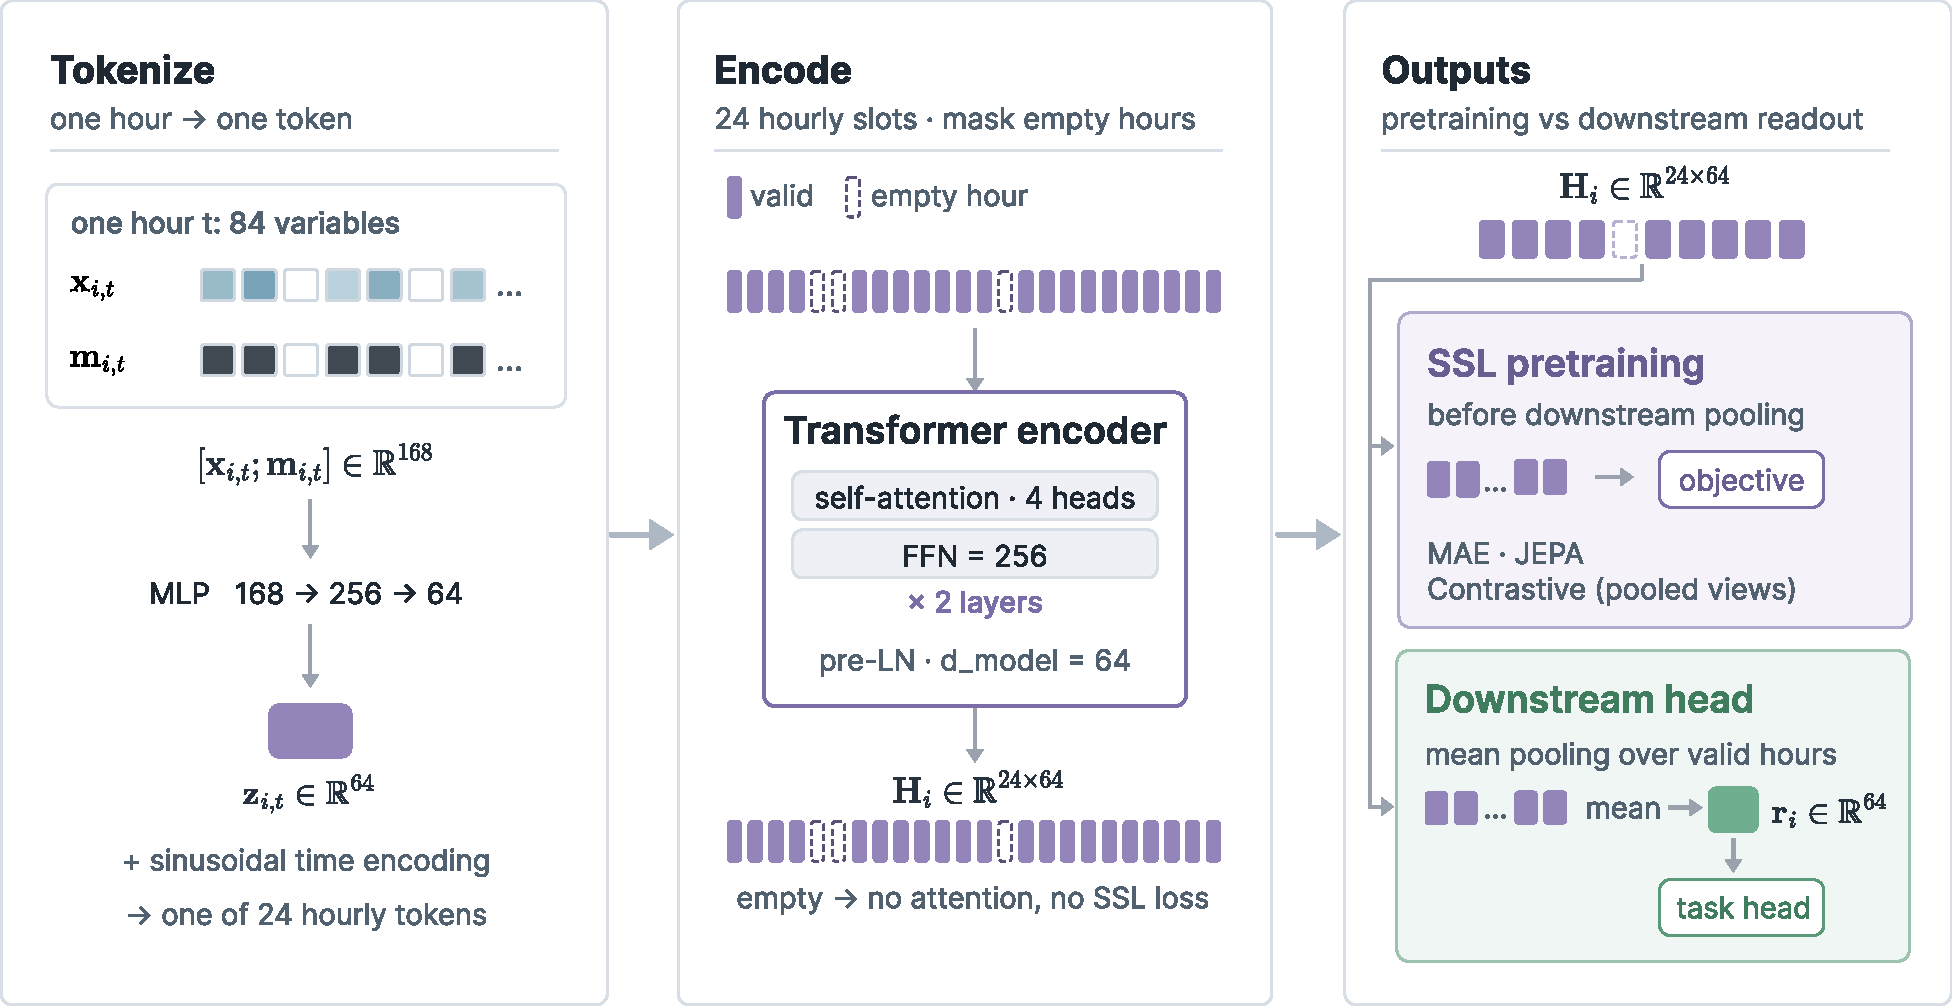
\includegraphics[width=\textwidth]{diagrams/fig03-encoder-tokenization.pdf}}
\end{figure*}

\subsection{Downstream Protocols}

Figure~\ref{fig:protocol-ab} separates frozen probing from full fine-tuning. Both use the same final pretraining encoder but differ in trainable scope, head capacity, learning rate, and epoch cap. These are two evaluation protocols, not a freeze-only ablation. The separate checkpoint diagnostic changes the SSL encoder selection policy only within its stated scope.

\begin{figure*}[p]
\floatconts{fig:protocol-ab}
{\caption{Reference downstream protocols. The displayed 50 and 100 epochs are maximum budgets. Validation patience is ten epochs. Protocol A trains a linear head. Protocol B adapts the encoder and a width-64 MLP head. Validation selects each downstream checkpoint before one test evaluation. Both start from final-epoch SSL weights.}}
{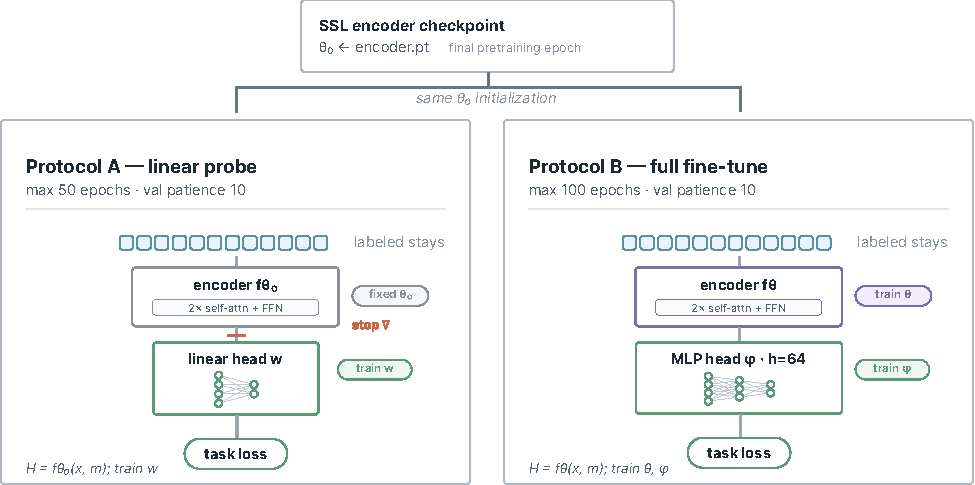
\includegraphics[width=\textwidth]{diagrams/fig05-protocol-ab.pdf}}
\end{figure*}

\subsection{Task Definitions and Test Support}

Tables~\ref{tab:task-definitions} and~\ref{tab:test-support} give the target rules and exported test support.

\begin{table*}[htbp]
\floatconts
  {tab:task-definitions}
  {\caption{Downstream task contract. All tasks use hours 0--24 as model input.}}
  {\scriptsize
  \begin{tabular}{p{.12\textwidth}p{.12\textwidth}p{.22\textwidth}p{.25\textwidth}l}
  \toprule
  Task & Horizon after input & Target & Null-label rule & Primary metric \\
  \midrule
  24h mortality & hours 24--48 & death in forward day & death in hours 0--24 & AUPRC \\
  Hosp. mortality & after hour 24 & death before discharge & death in hours 0--24 & AUPRC \\
  AKI & hours 24--48 & creatinine-defined KDIGO $\geq1$ & missing baseline/forward evidence & AUPRC \\
  Remaining LOS & after hour 24 & ICU LOS minus one day, clipped at 0 & none & Absolute error (days) \\
  \bottomrule
  \end{tabular}}
\end{table*}

\begin{table*}[htbp]
\floatconts
  {tab:test-support}
  {\caption{Mean test support across the five patient splits. Positive counts and prevalence apply to classification tasks.}}
  {\scriptsize
  \begin{tabular}{llrrr}
\toprule
Data & Task & Test samples & Positive & Prevalence \\
\midrule
Combined & 24h mortality & 30,863.4 & 492.4 & 0.0160 \\
Combined & Hospital mortality & 30,869.0 & 3,135.8 & 0.1016 \\
Combined & AKI & 21,724.0 & 3,565.2 & 0.1641 \\
Combined & Remaining LOS & 31,092.2 & -- & -- \\
eICU-CRD & 24h mortality & 19,788.6 & 315.2 & 0.0159 \\
eICU-CRD & Hospital mortality & 19,788.6 & 1,823.8 & 0.0922 \\
eICU-CRD & AKI & 13,297.4 & 1,850.0 & 0.1391 \\
eICU-CRD & Remaining LOS & 19,966.4 & -- & -- \\
MIMIC-IV & 24h mortality & 11,150.0 & 185.4 & 0.0166 \\
MIMIC-IV & Hospital mortality & 11,157.0 & 1,310.0 & 0.1174 \\
MIMIC-IV & AKI & 8,423.2 & 1,710.6 & 0.2031 \\
MIMIC-IV & Remaining LOS & 11,194.8 & -- & -- \\
\bottomrule
\end{tabular}
}
\end{table*}

\subsection{Objective and Downstream Configuration}

\begin{table*}[htbp]
\floatconts
  {tab:objective-details}
  {\caption{Objective-specific modules and transferred capacity. Shared settings are listed in Section~\ref{sec:setup}.}}
  {\scriptsize
  \begin{tabular}{llllrr}
  \toprule
  Objective & Geometry & Learning target & Auxiliary module & Trainable & Transferred \\
  \midrule
  \MAE{} & random masked hours & observed normalized cells & Transformer decoder & 269,460 & 159,808 \\
  \JEPA{} & up to three masked blocks & EMA target embeddings & predictor + target encoder & 189,440 & 159,808 \\
  Contrastive & complementary views & instance agreement & projection MLP & 193,408 & 159,808 \\
  \bottomrule
  \end{tabular}}
\end{table*}

The \JEPA{} target encoder adds a non-trainable 159,808-parameter copy. Its EMA coefficient increases linearly from .999 to 1.0. The predictor has width 32, two layers, four heads, and feed-forward width 128. The contrastive projection has hidden width 256 and output width 64. All auxiliary modules are discarded before downstream evaluation.

\subsection{Retained Features and Preprocessing}

The ordered 84 RICU concept identifiers below define the model schema, not a claim that each is observed in both sources. Source-specific missingness remains explicit. Extraction uses RICU 0.6.3 concept definitions and unit conversions, requested at one-hour intervals. Concept-specific aggregation is inherited from RICU. Python tensorization neither quantizes values nor forward-fills across hours. It uses the observed training-partition mean and sample SD per feature. SD is floored at $10^{-6}$. Features absent in training retain a zero mean and unit SD. Missing values become zero after normalization. Low-label subsets retain the full training-partition normalizer. The code repository includes extraction scripts and the complete input blocklist, including direct LOS, future vasopressor-duration, and derived score features.

\begin{quote}\footnotesize
\texttt{abx}, \texttt{adh\_rate}, \texttt{alb}, \texttt{alp}, \texttt{alt}, \texttt{ast}, \texttt{avpu}, \texttt{basos}, \texttt{be}, \texttt{bicar}, \texttt{bili}, \texttt{bili\_dir}, \texttt{bnd}, \texttt{bun}, \texttt{ca}, \texttt{cai}, \texttt{ck}, \texttt{ckmb}, \texttt{cl}, \texttt{cort}, \texttt{crea}, \texttt{crp}, \texttt{dbp}, \texttt{dex}, \texttt{dobu\_rate}, \texttt{dopa\_rate}, \texttt{egcs}, \texttt{eos}, \texttt{epi\_rate}, \texttt{esr}, \texttt{etco2}, \texttt{ett\_gcs}, \texttt{fgn}, \texttt{fio2}, \texttt{glu}, \texttt{hba1c}, \texttt{hbco}, \texttt{hct}, \texttt{hgb}, \texttt{hr}, \texttt{inr\_pt}, \texttt{ins}, \texttt{k}, \texttt{lact}, \texttt{lymph}, \texttt{map}, \texttt{mch}, \texttt{mchc}, \texttt{mcv}, \texttt{mech\_vent}, \texttt{methb}, \texttt{mg}, \texttt{mgcs}, \texttt{na}, \texttt{neut}, \texttt{norepi\_rate}, \texttt{o2sat}, \texttt{pco2}, \texttt{ph}, \texttt{phn\_rate}, \texttt{phos}, \texttt{plt}, \texttt{po2}, \texttt{pt}, \texttt{ptt}, \texttt{rass}, \texttt{rbc}, \texttt{rdw}, \texttt{resp}, \texttt{samp}, \texttt{sao2}, \texttt{sbp}, \texttt{spo2}, \texttt{supp\_o2}, \texttt{tco2}, \texttt{temp}, \texttt{tgcs}, \texttt{tnt}, \texttt{tri}, \texttt{urine}, \texttt{vent\_end}, \texttt{vent\_start}, \texttt{vgcs}, \texttt{wbc}.
\end{quote}

\subsection{Exact Losses and Baseline Configuration}

MAE minimizes squared reconstruction error averaged over observed feature cells at masked non-empty hours. JEPA uses elementwise squared error between predictions and layer-normalized stop-gradient target embeddings, averaged across valid target dimensions/hours. Its EMA coefficient rises from .999 to 1.0. EMA and target normalization are not evidence of collapse prevention. Core contrastive learning uses cosine similarity between normalized projected stay vectors. Each of the $2B$ view embeddings has its paired view as positive and the other non-self batch views in an NT-Xent denominator, at temperature .07. Losses differ in target space and reduction unit.

Binary mortality and AKI use two-logit cross entropy with label smoothing .1 and class weights $w_c=\sqrt{n/(2n_c)}$ from the labeled training subset. They are classification tasks, not time-to-event regression. LOS uses untransformed remaining days, squared-error training loss, and absolute-error validation/test evaluation. The constant median is the empirical training-label median evaluated on the test labels. It is not fitted on the test set.

GRU-D has hidden width 64, one recurrent layer, dropout .1, learned input/hidden decay, and the full-fine-tuning head and schedule. XGBoost receives eight summaries per variable: observed mean, SD, minimum, maximum, first, last, count, and fraction, for 672 inputs. It uses at most 1,000 trees, depth 6, learning rate .1, row/column subsampling .8, minimum child weight 1, and validation patience 20. Classification uses the native negative/positive class ratio and validation \texttt{aucpr}. Regression uses the squared-error objective and validation \texttt{mae}. These differ from neural weighting and average-precision implementation. All test AUPRC values use the shared evaluation definition. Exported per-run scientific configurations, rather than current defaults, are the reproduction reference.

\subsection{Full Baseline Matrix}

Table~\ref{tab:baseline-full} reports all full-label contextual baseline comparisons.

\begin{table*}[htbp]
\floatconts
  {tab:baseline-full}
  {\caption{Full-data contextual baselines and the best SSL mean. Classification rows report AUPRC (higher is better). LOS rows report absolute error in days (lower is better). Bold marks the best unrounded mean per row. All entries average five seeds.}}
  {\scriptsize
  \begin{tabular}{llrrrrl}
\toprule
Data & Endpoint & GRU-D & XGBoost & Supervised & Best SSL & SSL method \\
\midrule
Combined & 24h mortality & \textbf{0.422} & 0.374 & 0.389 & 0.409 & MAE \\
Combined & Hospital mortality & 0.527 & 0.525 & 0.518 & \textbf{0.531} & MAE \\
Combined & AKI & 0.630 & \textbf{0.668} & 0.652 & 0.626 & JEPA \\
Combined & Remaining LOS & 2.174 & 2.340 & 2.190 & \textbf{2.118} & MAE \\
eICU-CRD & 24h mortality & \textbf{0.397} & 0.315 & 0.351 & 0.377 & MAE \\
eICU-CRD & Hospital mortality & 0.484 & 0.482 & 0.474 & \textbf{0.495} & MAE \\
eICU-CRD & AKI & 0.510 & \textbf{0.569} & 0.554 & 0.519 & MAE \\
eICU-CRD & Remaining LOS & 2.003 & 2.163 & 1.997 & \textbf{1.964} & MAE \\
MIMIC-IV & 24h mortality & \textbf{0.480} & 0.402 & 0.449 & 0.456 & Contrastive \\
MIMIC-IV & Hospital mortality & 0.577 & 0.577 & 0.565 & \textbf{0.579} & MAE \\
MIMIC-IV & AKI & 0.661 & \textbf{0.729} & 0.693 & 0.667 & MAE \\
MIMIC-IV & Remaining LOS & 2.394 & 2.613 & 2.397 & \textbf{2.359} & Contrastive \\
\bottomrule
\end{tabular}
}
\end{table*}

\section{Secondary Analyses}
\label{app:secondary}

\subsection{Paired Classification Differences}

\begin{figure*}[htbp]
\floatconts
  {fig:seed-differences}
  {\caption{Matched-seed classification AUPRC differences, MAE minus comparator. Positive values favor MAE. Points are mean paired differences. Bars span the five observed differences, not a confidence interval. Supervised appears only for full fine-tuning.}}
  {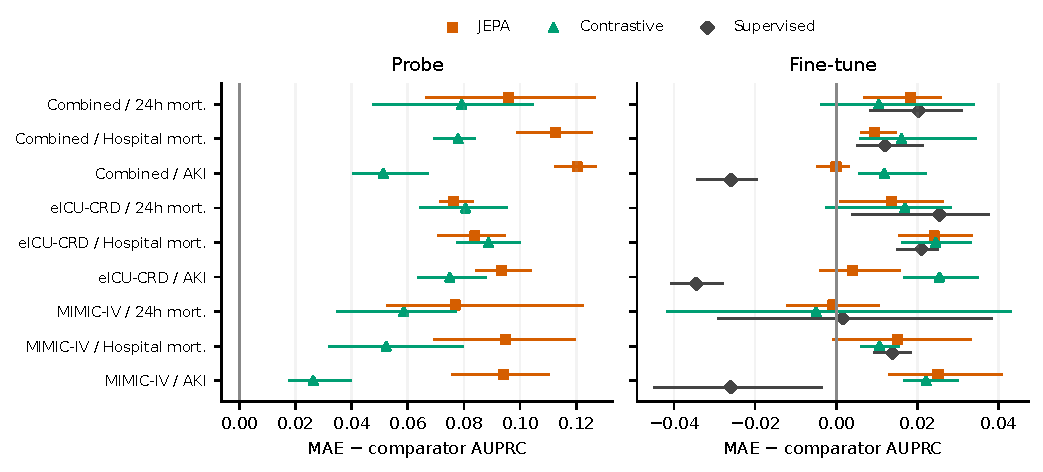
\includegraphics[width=.92\textwidth]{generated/seed-variance.pdf}}
\end{figure*}

\subsection{Label Efficiency}

\begin{figure*}[htbp]
\floatconts
  {fig:label-efficiency}
  {\caption{Hospital-mortality label efficiency under full fine-tuning, including the supervised Transformer at each label fraction. Points are five-seed means. Bars are sample SD across seeds. Only training labels are reduced.}}
  {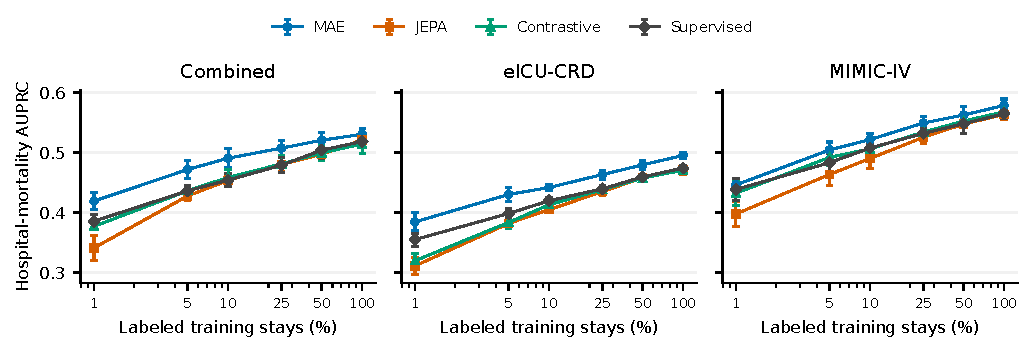
\includegraphics[width=.94\textwidth]{generated/label-efficiency.pdf}}
\end{figure*}

Only the labeled training subset is reduced. Validation and test partitions remain unchanged. Fractions are selected deterministically by seed without class stratification and need not be nested. Hospital mortality uses 1\%, 5\%, 10\%, 25\%, 50\%, and the full-label reference. Twenty-four-hour mortality starts at 5\%. AKI and LOS use 10\% and full-label references. Each cell contains five seeds.


At the lowest exported fraction for \Combined{} hospital mortality (1\%), fine-tuned AUPRC means are .419 for \MAE{}, .341 for \JEPA{}, .377 for contrastive learning, and .386 for supervised training. At 5\% labels for 24-hour mortality, the corresponding means are .277, .241, .245, and .267. When full-label references are included, MAE leads 39/45 fine-tuning cells among SSL methods, 35/45 with supervised included, and 37/45 probe cells among SSL methods. Section~\ref{sec:results} instead counts only fractions below 100\%. Comparator sets and denominators must be stated together.

\begin{table*}[htbp]
\floatconts{tab:low-label}{\caption{Lowest exported label fractions, full fine-tuning. MAE and supervised means use AUPRC for classification and absolute error in days for LOS. $\Delta$ is MAE minus supervised. Positive favors MAE only for classification. SD is computed from five paired differences, not from independent error propagation.}}
{\scriptsize\begin{tabular}{lllrrrr}
\toprule
Data & Task & Labels & MAE & Supervised & $\Delta$ mean & $\Delta$ SD \\
\midrule
Combined & 24h mortality & 5\% & 0.277 & 0.267 & 0.010 & 0.027 \\
Combined & Hospital mortality & 1\% & 0.419 & 0.386 & 0.033 & 0.012 \\
Combined & AKI & 10\% & 0.514 & 0.507 & 0.006 & 0.021 \\
Combined & Remaining LOS & 10\% & 2.229 & 2.252 & -0.023 & 0.024 \\
eICU-CRD & 24h mortality & 5\% & 0.260 & 0.248 & 0.011 & 0.015 \\
eICU-CRD & Hospital mortality & 1\% & 0.385 & 0.355 & 0.029 & 0.019 \\
eICU-CRD & AKI & 10\% & 0.405 & 0.411 & -0.006 & 0.009 \\
eICU-CRD & Remaining LOS & 10\% & 2.067 & 2.081 & -0.014 & 0.034 \\
MIMIC-IV & 24h mortality & 5\% & 0.294 & 0.268 & 0.026 & 0.041 \\
MIMIC-IV & Hospital mortality & 1\% & 0.446 & 0.439 & 0.008 & 0.021 \\
MIMIC-IV & AKI & 10\% & 0.565 & 0.549 & 0.016 & 0.012 \\
MIMIC-IV & Remaining LOS & 10\% & 2.494 & 2.490 & 0.004 & 0.071 \\
\bottomrule
\end{tabular}
}
\end{table*}

\subsection{Cross-Database Adaptation}

Cross-database rows pretrain on one database and then fully fine-tune using labels from the other. They are off-diagonal adaptation results, not zero-shot validation. No same-source comparator was launched inside this analysis slice. MAE has the best mean primary metric on all four \MIMIC{}-to-\EICU{} tasks and three of four reverse-direction tasks. Contrastive learning leads reverse-direction 24-hour mortality (\tableref{tab:transfer}). These rankings do not establish a benefit over target-domain pretraining or a general transfer advantage.

\begin{table*}[htbp]
\floatconts
  {tab:transfer}
  {\caption{Cross-database full-fine-tuning means over five seeds. Classification uses AUPRC. LOS uses absolute error in days. Bold marks the best unrounded mean within each row.}}
  {\scriptsize
  \begin{tabular}{llllrrr}
\toprule
Pretrain & Target & Task & Metric & MAE & JEPA & Contrastive \\
\midrule
eICU-CRD & MIMIC-IV & 24h mortality & AUPRC & 0.447 & 0.453 & \textbf{0.454} \\
eICU-CRD & MIMIC-IV & Hospital mortality & AUPRC & \textbf{0.572} & 0.559 & 0.564 \\
eICU-CRD & MIMIC-IV & AKI & AUPRC & \textbf{0.646} & 0.643 & 0.627 \\
eICU-CRD & MIMIC-IV & Remaining LOS & Abs. error & \textbf{2.389} & 2.390 & 2.403 \\
MIMIC-IV & eICU-CRD & 24h mortality & AUPRC & \textbf{0.372} & 0.367 & 0.354 \\
MIMIC-IV & eICU-CRD & Hospital mortality & AUPRC & \textbf{0.485} & 0.477 & 0.476 \\
MIMIC-IV & eICU-CRD & AKI & AUPRC & \textbf{0.5323} & 0.5205 & 0.5322 \\
MIMIC-IV & eICU-CRD & Remaining LOS & Abs. error & \textbf{1.966} & 1.987 & 1.998 \\
\bottomrule
\end{tabular}
}
\end{table*}

\subsection{Encoder Capacity and Subgroup Auditing}
\label{app:capacity-subgroups}

The capacity analysis compares MAE and supervised Transformers on \MIMIC{} 24-hour mortality at 5\%, 10\%, and 50\% labels. Under full fine-tuning, medium and large MAE models exceed their corresponding supervised models by .013--.028 mean AUPRC across the six size--fraction cells, each with five seeds. This one-task, one-database slice does not test larger JEPA or contrastive encoders and cannot establish a general scaling rule.

Subgroup auditing records maximum-minus-minimum performance gaps across eligible gender, age, and race groups, requiring at least 50 unique patients and a defined metric per group. In the core full-label classification cells, across-seed mean AUPRC gaps range from .004 to .095 for gender, .033 to .172 for age, and .080 to .513 for race. These ranges cover 63 gender cells, 63 age cells, and 42 race cells. Race metrics are unavailable for \EICU{}, and \Combined{} race analyses use \MIMIC{}-origin records. A 50-patient threshold does not ensure enough positive outcomes for stable AUPRC. These summaries describe gaps without ranking methods by fairness or attributing their causes. They do not assess intersectional groups or subgroup calibration.

\subsection{TS2Vec Context}

\label{app:ts2vec}

Our TS2Vec-style extension retains the SLICES Transformer and value--mask interface, rather than the original dilated convolutional encoder. It adds Gaussian noise of SD .01 to observed values, independently masks half the hours in each view, and uses no temporal crop in the reference configuration. A width-256/output-64 projection precedes temperature-.05 NT-Xent over overlapping timestep pairs. Negatives combine other times and other instances in one denominator. This differs from original TS2Vec's separate temporal and instance losses. Four max-pooling scales (1, 2, 4, 8 hours) use mask-aware validity and an average over active scales. Thus these results characterize this extension, not original TS2Vec's performance \citep{yue2022ts2vec}.

\begin{table*}[htbp]
\floatconts
  {tab:ts2vec}
  {\caption{TS2Vec-style extension versus the core contrastive implementation. Entries count dataset--task cells with the better unrounded mean among 12 cells per protocol.}}
  {\begin{tabular}{lrr}
\toprule
Protocol & TS2Vec-style & Core contrastive \\
\midrule
Fine-tune & 8 & 4 \\
Probe & 0 & 12 \\
\bottomrule
\end{tabular}
}
\end{table*}

The full-fine-tuning split is task dependent. For example, TS2Vec is higher on \MIMIC{} 24-hour mortality (.465 versus .456), while core contrastive is lower on \MIMIC{} LOS (2.359 versus 2.370). Under probing, the core contrastive mean is better in every cell, including \MIMIC{} AKI (.478 versus .441) and LOS (2.592 versus 2.722). These five-seed differences do not establish equivalence or general dominance.

\subsection{Demonstrated Extension Workflow}
\label{app:extension-workflow}

\begin{figure*}[htbp]
\floatconts
  {fig:benchmark}
  {\caption{\SLICES{} benchmark. The reusable path from fixed specification through objective extension and encoder transfer to auditable results. Comparison checks enforce declared settings and export coverage. They do not prove that a training run used its declared private data. Objective-specific modules and compute remain different.}}
  {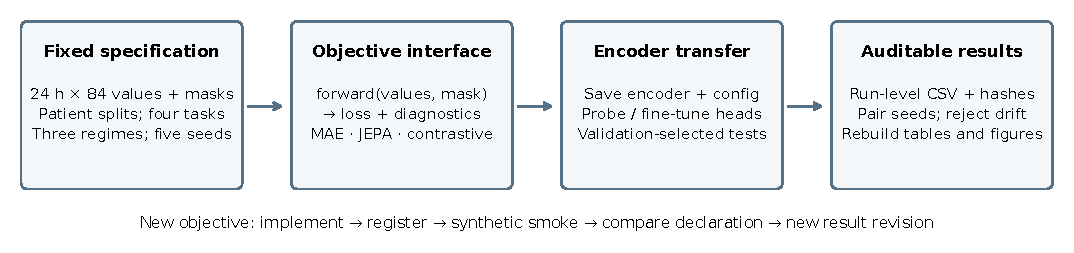
\includegraphics[width=\textwidth]{generated/benchmark-overview.pdf}}
\end{figure*}

The code repository's \texttt{TS2VEC\_CASE.md} gives a runnable path through the existing extension. Objective code, its configuration dataclass, registry entries, encoder-compatibility entry, and SSL YAML define the replaceable components. Clinical preprocessing, feature order, the shared encoder, final-epoch transfer, task heads, protocol schedules, primary metrics, and result identities define the retained scientific contract. The case adds execution and reporting code. It does not alter the objective or the frozen results.

The command \texttt{extension.py --out extension-output} uses 80 artificial patients, the shared 70/15/15 split function, train-only normalization, and the full 159,808-parameter encoder. It runs two SSL epochs and two epochs for each synthetic binary/regression task under each protocol. These reduced budgets, artificial targets, and single seed are recorded as departures from the scientific contract. Checks cover exact v3 encoder transfer, discarded projection weights, unchanged frozen parameters, updated fine-tuned parameters, validation selection, and exact test-checkpoint reload. Synthetic metrics remain in a separate output file. The frozen report instead joins 120 existing TS2Vec runs to their matched core-contrastive runs, retaining means, sample SDs, paired differences, and configuration IDs.

Validation records distinguish implementation assistance and failed attempts from successful execution of the extracted archive's instructions. This is a development-agent check on a fresh environment, with no independent human reuse study. It does not test credentialed extraction, clinical label construction, or historical numerical retraining equivalence.

\subsection{Post-Hoc Random-Encoder Diagnostic}

The random diagnostic contains 40 task--dataset--seed rows over \MIMIC{} and \EICU{}. It freezes an untrained instance of the same default Transformer and trains only the linear task head from cached embeddings. Pairing those rows with the three core SSL probes gives 120 comparisons. The random probe is worse in 118. The exceptions are both against \JEPA{} on \EICU{}: +.0006 AUPRC for AKI and +.0013 for 24-hour mortality, each in one run. This analysis was produced after the frozen export and was not part of the core family. The new raw/mask control below is another separate diagnostic.


\subsection{JEPA, Checkpoint, and Hyperparameter Diagnostics}
\label{app:diagnostics}

The separate JEPA diagnostic covers all 15 core pretraining runs. Across logged steps, the minimum target representation SD is .3664 and maximum mean pairwise cosine is .8209. The mean final SD is 1.1695. These statistics cannot rule out partial collapse or establish downstream quality. The historical checkpoint audit covers 45 core pretraining encoders. Core downstream runs use the final 100-epoch encoder. Retained JEPA validation-checkpoint files are from epochs 3--5. These are not final encoders and do not mean training ended early.

The new checkpoint diagnostic completes 60 frozen probes, or 30 final-versus-best-SSL-validation pairs, over the three core objectives, five seeds, and MIMIC-IV hospital mortality and LOS. Both arms use the same cached CPU implementation, patient splits, train-only normalization, head initialization and batch RNG. Linear heads use the reference AdamW/cosine settings, validation patience and epoch cap. LOS trains with squared error and selects/reports absolute error. Validation alone selects the head, with the earliest epoch retained on a tie. The test set is evaluated once afterward. Producer checks matched all 30 encoder hashes to the frozen audit. The public audit reconstructs paired statistics and all 60 selections from saved validation histories.

\begin{table*}[htbp]
\floatconts{tab:checkpoint-sensitivity}
{\caption{Separate MIMIC-IV cached CPU probe diagnostic. Mean $\pm$ sample SD over five seeds. Mortality uses AUPRC. LOS uses absolute error in days. $\Delta$ is best-SSL-validation minus rerun-final. Brackets give the observed paired range. These final-arm values are reruns, not substituted historical scores.}}
{\scriptsize\begin{tabular}{llrlll}
\toprule
Task & Encoder & $n$ & Rerun final & Best SSL val. & $\Delta$ mean [range] \\
\midrule
Hospital mortality & MAE & 5 & 0.5093 $\pm$ 0.0135 & 0.5096 $\pm$ 0.0139 & +0.0003 [-0.0009, +0.0019] \\
Hospital mortality & JEPA & 5 & 0.4139 $\pm$ 0.0196 & 0.3733 $\pm$ 0.0094 & -0.0406 [-0.0563, -0.0166] \\
Hospital mortality & Contrastive & 5 & 0.4574 $\pm$ 0.0236 & 0.4573 $\pm$ 0.0236 & -0.0001 [-0.0003, +0.0000] \\
Remaining LOS & MAE & 5 & 2.7655 $\pm$ 0.0651 & 2.7644 $\pm$ 0.0628 & -0.0011 [-0.0047, +0.0019] \\
Remaining LOS & JEPA & 5 & 2.6758 $\pm$ 0.0903 & 2.9396 $\pm$ 0.0916 & +0.2638 [+0.1909, +0.3689] \\
Remaining LOS & Contrastive & 5 & 2.5946 $\pm$ 0.0662 & 2.5949 $\pm$ 0.0655 & +0.0003 [-0.0009, +0.0018] \\
\bottomrule
\end{tabular}
}
\end{table*}

JEPA worsens in all five seeds on both tasks (Table~\ref{tab:checkpoint-sensitivity}). MAE leads mortality and contrastive leads LOS under both policies in every seed, while JEPA's LOS mean rank drops from second to third. Rerun-final cell means differ from historical means by -.001018 to -.000106 AUPRC and -.003616 to +.010286 LOS days. The largest absolute per-seed LOS deviation is .090066 days. Cached CPU execution and dedicated paired RNG differ from historical GPU/Lightning execution. This diagnostic took 19.60 wall minutes on CPU, with no failed or timed-out workers. It supports scoped checkpoint sensitivity, not equivalence, general rank stability, or conclusions about other databases or full fine-tuning.

Table~\ref{tab:hp} contains only MIMIC-IV 24-hour mortality, full fine-tuning, full labels, and five seeds per level. Learning-rate values are upstream pretraining rates. Mask sweeps change their respective objective's mask ratio. The largest within-objective range of mean AUPRC across tested levels is .018039. This targeted slice establishes neither hyperparameter insensitivity nor objective-specific optimal tuning. Its test-set rankings are not used to select a new headline configuration.

\begin{table*}[htbp]
\floatconts{tab:hp}{\caption{Existing targeted pretraining hyperparameter diagnostics. Downstream AUPRC mean and sample SD, $n=5$ per level.}}
{\scriptsize\begin{tabular}{lllrr}
\toprule
Sweep & Objective & Level & AUPRC & SD \\
\midrule
lr sensitivity & Contrastive & 0.0002 & 0.462 & 0.035 \\
lr sensitivity & Contrastive & 0.0005 & 0.465 & 0.033 \\
lr sensitivity & Contrastive & 0.002 & 0.459 & 0.042 \\
lr sensitivity & JEPA & 0.0002 & 0.467 & 0.028 \\
lr sensitivity & JEPA & 0.0005 & 0.461 & 0.049 \\
lr sensitivity & JEPA & 0.002 & 0.449 & 0.053 \\
lr sensitivity & MAE & 0.0002 & 0.462 & 0.047 \\
lr sensitivity & MAE & 0.0005 & 0.451 & 0.051 \\
lr sensitivity & MAE & 0.002 & 0.457 & 0.050 \\
mask ratio sensitivity & JEPA & 0.3 & 0.454 & 0.057 \\
mask ratio sensitivity & JEPA & 0.75 & 0.447 & 0.029 \\
mask ratio sensitivity & MAE & 0.3 & 0.464 & 0.033 \\
mask ratio sensitivity & MAE & 0.75 & 0.447 & 0.035 \\
view mask sensitivity & Contrastive & 0.3 & 0.460 & 0.035 \\
view mask sensitivity & Contrastive & 0.75 & 0.447 & 0.061 \\
\bottomrule
\end{tabular}
}
\end{table*}

\subsection{New Raw-Input and Mask-Only CPU Control}
\label{app:raw}

This post-hoc diagnostic uses only MIMIC-IV hospital mortality and the five canonical patient splits. A linear logistic classifier receives either 2,016 flattened mask entries or those entries plus 2,016 normalized values. Normalization uses the same full-cohort training partition. Task labels are filtered after patient assignment. Fixed SGD uses logistic loss, $L_2$ coefficient $10^{-4}$, the library's optimal learning-rate schedule, square-root-balanced sample weights, and 20 epochs. The epoch with highest validation average precision is evaluated once on the test set. No label smoothing or hyperparameter search is used. The implementation and input-file SHA256 values are recorded separately.

Test AUPRC is .301 (.025) for masks and .404 (.013) for values plus masks, mean (sample SD). Mean test support is 11,157 stays and 1,310 deaths. Total wall time is 136 seconds on a CPU limited to two threads, including both representations and all five seeds, under a 900-second hard timeout. Every mask-only run selects epoch 20, so further optimization could improve this control. The result does not establish the performance of an optimized raw-input model, nor does it isolate SSL gains from differences in optimization, regularization, input dimension, or head training.

\section{Evidence and Reproducibility Boundary}
\label{app:reproducibility}

The frozen evidence bundle used for the paper contains:
\begin{itemize}
  \item an aggregate result table with one row per scientific cell and seed summaries.
  \item a per-seed table used for matched differences and coverage checks.
  \item long-form metrics and retained diagnostic test outputs.
  \item label-efficiency, classical-context, and TS2Vec comparison tables.
  \item an evidence manifest recording row counts, schemas, analysis revision, and source hashes.
\end{itemize}

The core audit filter is: core SSL analysis, default model size, full label fraction, the three data regimes, four tasks, and the two adaptation protocols. It yields 84 aggregate rows with five seeds each and 420 per-seed rows. The random-encoder diagnostic is stored separately and is not merged into the frozen core ranking. No patient-level row is included in the paper source or code repository.

The code repository also includes \texttt{thesis-coverage-evidence.json}, with source hashes and aggregate cells for the capacity, subgroup, and LOS secondary-metric summaries. The paper source includes LaTeX, generated table fragments and vector figures, a bibliography, and the official class/style files. It builds with PDF\LaTeX{} and BibTeX through \texttt{latexmk}.

\end{document}
